\documentclass[a4paper]{article}
\usepackage[utf8]{inputenc}
\usepackage[T1]{fontenc}
\usepackage[pdftex]{graphicx}
\usepackage{fancyhdr}
\usepackage{lscape}
\usepackage{color}
\usepackage{qtree}
\usepackage[english]{babel}
\usepackage{graphicx}
\usepackage[colorinlistoftodos]{todonotes}
\usepackage{listings}
\usepackage{color}
\usepackage{changepage}
\usepackage[margin=1in]{geometry}
\definecolor{codegreen}{rgb}{0,0.6,0}
\definecolor{codegray}{rgb}{0.5,0.5,0.5}
\definecolor{codepurple}{rgb}{0.58,0,0.82}
\definecolor{backcolour}{rgb}{0.95,0.95,0.92}
\usepackage[parfill]{parskip}

 \lstdefinestyle{mystyle}{
 	backgroundcolor=\color{backcolour},   
 	commentstyle=\color{codegreen},
 	keywordstyle=\color{magenta},
 	numberstyle=\tiny\color{codegray},
 	stringstyle=\color{codepurple},
 	basicstyle=\footnotesize,
 	breakatwhitespace=false,         
 	breaklines=true,                 
 	captionpos=b,                    
 	keepspaces=true,                 
 	numbers=left,                    
 	numbersep=5pt,                  
 	showspaces=false,                
 	showstringspaces=false,
 	showtabs=false,                  
 	tabsize=2
 }
 
\lstset{
	style=mystyle,
	inputencoding=utf8,
	extendedchars=true,
	literate={á}{{\'a}}1 {ã}{{\~a}}1 {é}{{\'e}}1,
	escapechar=\&
}
\title{Algorithmique et structures de données : Mission 3}
\date{30 octobre 2014}
\author{Groupe 1.2: Ivan Ahad - Jérôme Bertaux - Rodolphe Cambier \\ 
	Baptiste Degryse - Wojciech Grynczel - Charles Jaquet}



\begin{document}
\maketitle



Rapport écrit par Ivan Ahad, Rodolphe Cambier et Charles Jacquet

\subsection*{Introduction}
Pour ce programme, nous avions à implémenter une map pour contenir les informations sur le classement de magasines. Chaque magasine contient plusieurs informations, comme son nom (qui le distingue des autres), sa note, etc.
Nous allons commencer par présenter le fonctionnement de notre programme, ensuite nous parlerons de l'évaluation des performances de celui-ci. Et nous terminerons par les tests que nous avons effectués.

\subsection*{Choix d'implémentations et fonctionnement}
La Main commence par créer un nouveau "Journal". Ensuite, il fait une boucle dans laquelle il demande à l'utilisateur un nom de journal à rechercher.
Et il recommence ces deux dernières opérations tant que l'utisateur ne veut plus continuer.
Pour ce qui est de la classe Journal, le constructeur prend plusieurs arguments. Le premier est l'index de la clé qui sera utilisée (c'est à dire, pour nous le nom avec l'index 1). Le deuxième est le nom du fichier et enfin le dernier est le délimiteur utilisé.\\
Fonctionnement du constructeur du journal:\\
Pour chaque ligne, il va faire un split avec le délimiteur rentré en argument. Ensuite, il va tester le nombre d'élements. S'il y en a pas suffisamment,  il rajoute alors un tableau vide à la fin car cela signifie qu'il n'y a rien après les délimiteurs. S'il y en a de trop, il check les guillemets pour remettre ensemble les tableaux qui ne devaient pas être séparés. Enfin Il rajoute l'élément à une map, déjà implémentée en java. Pour le rajout d'un élément, il utilise également la classe Entrée qui permet de lier les clés et les valeurs ensemble.

\section*{Evaluation des performances}

\subsection*{Complexité temporelle de la classe Entrée}

Le constructeur de la classe Entrée a une complexité en $\Theta(n)$ où n représente le nombre de clés contenues dans le tableau "cle[]". Le constructeur contient deux boucles "for" dont la première tournera exactement autant de fois qu'il y a de clés, et dont la deuxième tournera autant de fois que la différence entre le nombre de clés et de valeurs. Ainsi, nous prenons L valeur la plus grande (vu qu'il s'agit d'une addition de deux boucles) pour déterminer "n". 
\\
L'autre méthode dans la classe Entrée est la méthode "toString" dont la complexité sera de $\Theta(n)$ où n représente également le nombre de clés. 
\\
\subsection*{Complexité temporelle de la classe Journal et la classe JournalTest}

Tout d'abord, nous avons une première boucle while qui permet de lire le fichier avec lequel nous créons un journal. Cette boucle s'arrête dès que la ligne à lire est "null". Ainsi, la complexité temporelle de cette boucle est en $\Theta(n)$ où n représente le nombre de lignes du fichier à lire. 
\\
A l'intérieur de cette boucle, nous avons une boucle for avec deux conditions qui tournera exactement m fois, où m représente le nombre de fois où les deux conditions seront respectées. Ainsi, cette boucle a une complexité en $\Theta(m)$. 
\\
Enfin, à l'intérieur de ces deux boucles nous avons une troisième boucle dont la complexité est en $\Theta(p)$ où p représente le nombre de fois où la condition est respectée. 
Au final, cela correspond à une complexité de $\Theta(n*m*p)$
\\
Dans la classe de test "JournalTest", nous faisons appel à la méthode de création de journal, ainsi la complexité est la même que ci-dessus. 
\\
\subsection*{Complexité temporelle de la Main}

Au début de la Main nous faisons appel à la méthode permettant de créer un journal à partir d'un fichier. Comme décrite plus haute, la complexité de cet appel est donc en $\Theta(n*m*p)$. 
\\
La classe Main utilise ensuite un scanner pour pouvoir communiquer avec l'utilisateur. Notre programme est tel qu'on utilise une boucle while où l'utilisateur rentre une valeur "y" ou "Y" pour continuer à rentrer un nom de journl. La boucle s'arrête dès que l'utilisateur rentre une valeur autre que ces deux-ci. Ainsi, la complexité est en $\Theta(n)$ où n représente le nombre de fois où l'utilisateur a rentré "y" ou "Y", car toutes les autres opérations de la boucle se font en temps constant. 
\\
Comme nous prenons en compte la complexité la plus grande du programme, la complexité de la Main sera égale à la complexité de l'appel à la méthode permettant de créer un journal. 
\\
\section*{Les tests}

Nous avons testé le fonctionnement du programme grâce aux fichier \textit{Journal.csv} et grâce à la classe \textit{JournalTest.java}. Dans la Main, nous créons un objet \textit{JournalTest}, et nous testons, grâce aux fonctions définies dans cet objet, différents cas, notamment en plaçant une virgule à certains endroits critiques.


\subsection*{UML}
\centering
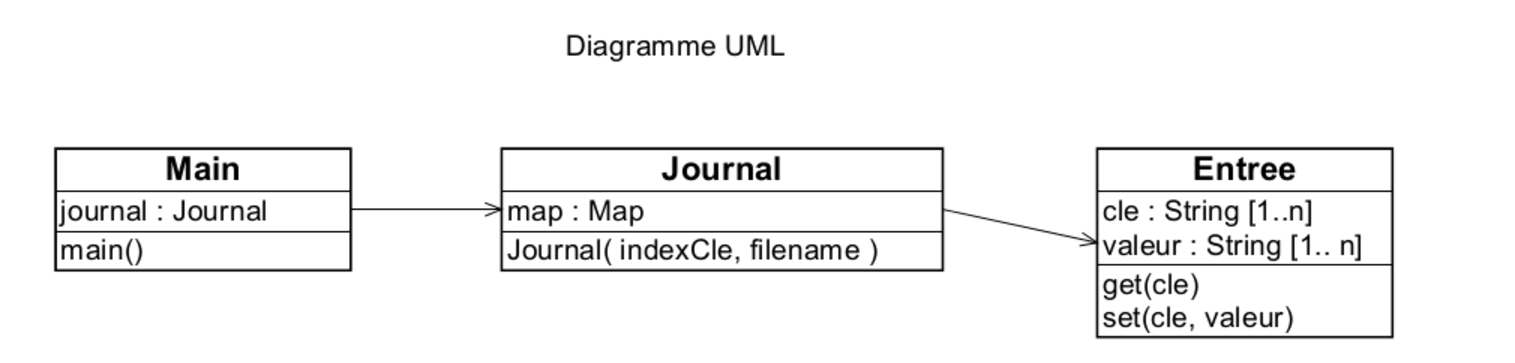
\includegraphics[scale=0.4]{DiagrammeUML.pdf}

\end{document}